\chapter{Implementierung}\label{ch:implementierung}
Das Projekt wurde in C++11 umgesetzt. Für die Erstellung einer Benutzeroberfläche wurde die QT5 Bibliothek verwendet \cite{qt5}.
Für verschiedene Algorithmen aus der Mustererkennung wurde die OpenCV2 Bibliothek genutzt \cite{opencv}. Außerdem verwenden wir CMake
als plattformunabhängiges Build-System \cite{cmake}. Für das Projekt haben wir zwei separate Anwendungen erstellt, den QViewer und das Auto-Train
Programm.

Die im nächsten Kapitel vorgestellten Ergebnisse wurden an Computer mit den Betriebssystem Archlinux erstellt, der den Linux-Kernel in Version 4.7.3 verwendet. Weiter wurde OpenCV in der Version 2.4.13, der C++ Compiler GCC in Version 6.2, CMake in der Version 3.6.2 und Qt in der Version 5.7 benutzt. Der Rechner besitzt einen 4-Kern Prozessor von AMD mit jeweils 2.8 GHz an Kapazität und einen Arbeitsspeicher von 8 GB. 

\begin{figure}[ht]
\begin{center}
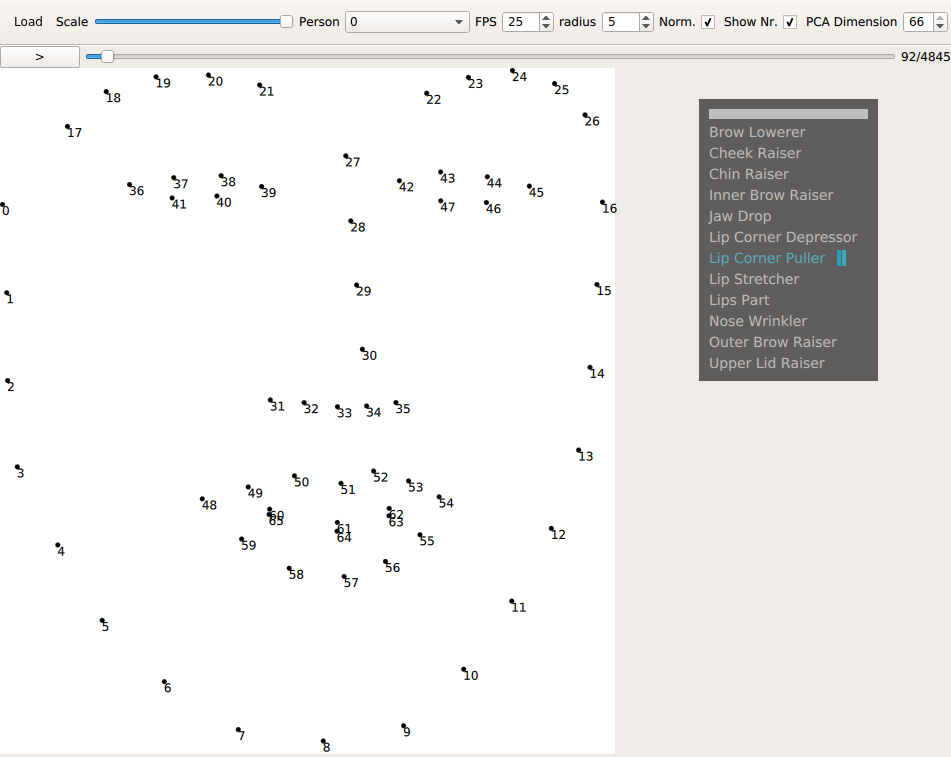
\includegraphics[width=0.6\textwidth]{qviewer.png}
\end{center}
\caption{Screenshot der QViewer Anwendung}
\label{fig:implementierung.QViewer}
\end{figure}

\section{QViewer}
Der QViewer ermöglicht uns eine Visualisierung der Eingabedaten.
Es ist eine in Qt geschrieben grafische Oberfläche, in der
die Landmark und Action Unit Dateien geladen werden können. 
Ein Nutzer kann dann eine Person auswählen und dessen Landmarks als Videos abspielen.
Dabei werden dann die Intensitäten der Action Units angezeigt. Auf Abbildung~\ref{fig:implementierung.QViewer} ist die Oberfläche des Programmes zu erkennen.
Zusätzlich können wir die Landmarks normalisieren. Weiter kann man durch PCA die Punkte auf einen neuen Raum mit weniger Dimensionen projezieren und dann wieder zurückprojezieren. Dadurch ist es möglich den Effekt von PCA zu veranschaulichen.
Der QViewer ist also insgesamt eine Hilfe um Landmarks, Action-Unit und einige hier beschriebenen Verfahren zu verstehen.
% was man sonst noch so machen kann



\section{Auto-Train}
Wie bereits in Kapitel \ref{ch:methodik} erwähnt, ist ein guter Klassifikator abhängig von der Wahl verschiedener Variablen, wie zum Beispiel
von der Auswahl der Features oder von den Parametern mit denen der Klassifikator trainiert wird.

Wünschenswert wäre ein Programm, das automatisch alle möglichen Kombinationen mitsamt der Vorverarbeitung und Evaluierung vornimmt und dabei alle nötigen Informationen, wie die Eigenvektoren bei PCA oder die gelernten Klassifikatoren, automatisch speichert.

Hier kommt das Programm Auto-Train ins Spiel. Das Programm liest aus einer JSON-Datei, wie sie im Anhang \ref{Anhang.config} zu finden ist, die gewünschte Konfiguration. Dazu zählen unter anderem die Schritte zur Vorverarbeitung der Landmarks und der extrahierten Features, als auch die zu verwendeten Feature-Extractoren. 

Zusätzlich zum Training kann das Programm, mithilfe einer etwas anderen JSON-Datei, dann gelernte Klassifikatoren und Parameter (wie z.B. Eigenvektoren der PCA) verwenden und die Performanz für eine Testmenge berechnen.
Der Einfachheit halber, wird die dafür benötigte JSON-Datei beim Training automatisch erstellt. Die Datei bedarf lediglich eines manuellen Eintrages für die zu evaluierenden Daten.

% \subsubsection{Feature-Extractor}
% Um möglichst viele Kombinationen von einzelnen Features miteinander kombinieren zu können, haben wir eine Feature-Extractor Aggregat
% Klasse erstellt, die es uns ermöglicht verschiedene Feature-Extractor aneinander zu koppeln und so kombinierte Features zu extrahieren.
% Kombiniert man beispielsweise die Extraktion der Orientierung zum Mittelpunkt, zusammen mit der Distanz zum Mittelpunkt, so erhält man
% pro Landmark zwei Features und damit pro Frame einen 132 elementigen Feature-Vektor \ref{Implementierung.Feature-Extractor}.\newline

% \begin{figure}
% \begin{center}
% \includegraphics[width=0.4\textwidth]{feature_extractor.png}
% \caption{UML-Diagramm der Feature-Extractor Klasse}
% \end{center}
% \label{Implementierung.Feature-Extractor}
% \end{figure}



% \begin{itemize}
%   \item Zum trainieren und evaluieren
%   \item Kurzes Wort zum Design von FeatureExtractor
%   \item Automatisches Speichern aller relevanten Dateien.
%   \item Erwähnung der JSON-Konfigurations-Datei
%     \begin{itemize}
%     \item Design von Processors
%   \end{itemize}
% \end{itemize}

%%% Local Variables:
%%% mode: latex
%%% TeX-master: "../../paper"
%%% End:
